\documentclass[10pt,a4paper]{article}
\usepackage[latin1]{inputenc}
\usepackage{amsmath}
\usepackage{amsfonts}
\usepackage{amssymb}
\usepackage{fullpage}
\usepackage{graphicx}

\begin{document}
\title{J.D. Jackson Problem 5.19}
\author{Josh Orndorff \\ admin@joshorndorff.com}
\maketitle

\section{Finding \textbf{H} and \textbf{B} using magnetic scalar potential}
Because there is no current in this problem, we are able to apply use the magnetic scalar potential method that Jackson derives in section 5.9.  the scalar potential is given by equation (5.100).
\begin{equation}
\Phi_M(r, \theta, z)=-\frac{1}{4\pi}\int_V\frac{\nabla'\cdot\mathbf{M}(\mathbf{x'})}{|\mathbf{x}-\mathbf{x'}|}\,\mathrm{d}V' + \frac{1}{4\pi}\oint_S\frac{\mathbf{\hat{n}'}\cdot\mathbf{M}(\mathbf{x'})}{|\mathbf{x}-\mathbf{x'}|}\,\mathrm{d}a'
\end{equation}

In this case, the magnetization is uniform and pointed along the $z$-axis, $\mathbf{M}=M_0\hat{z}$, so the first integral is zero, as is the sidewall's contribution to the second integral.  Further, by the cylindrical symmetry of the problem, we can see that the $H$-field at points on the $z$-axis will be oriented in the $\hat{z}$ direction.  So rather than expanding $|\mathbf{x}-\mathbf{x'}|^{-1}$ according to equation (3.70) and finding the scalar potential everywhere, finding it along the $z$-axis will suffice.
\begin{align}
\Phi_M(0, 0, z) &=\frac{1}{4\pi}\int_{top}\frac{\mathbf{\hat{z}}\cdot M_0\mathbf{\hat{z}}}{|\mathbf{x}-\mathbf{x'}|}\,\mathrm{d}a'+\frac{1}{4\pi}\int_{bottom}\frac{-\mathbf{\hat{z}}\cdot M_0\mathbf{\hat{z}}}{|\mathbf{x}-\mathbf{x'}|}\,\mathrm{d}a' \\
&=\frac{M_0}{4\pi}\int_0^{2\pi}\int_0^a\left[\frac{1}{\sqrt{(z-L)^2+r^2}}-\frac{1}{\sqrt{z^2+r^2}}\right]r\,\mathrm{d}r\,\mathrm{d}\phi \\
&=\frac{M_0}{2}\int_0^a\left[\frac{r}{\sqrt{(z-L)^2+r^2}}-\frac{r}{\sqrt{z^2+r^2}}\right]\,\mathrm{d}r \\
&=\frac{M_0}{2}\left[\sqrt{(z-L)^2+r^2}-\sqrt{z^2+r^2}\right]_0^a \\
&=\frac{M_0}{2}\left[\sqrt{(z-L)^2+a^2}-\sqrt{z^2+a^2}-\sqrt{(z-L)^2}+\sqrt{z^2}\right]
\end{align}

In order to simplify the latter two terms, we must break this potential into a piecewise function.  The latter two terms must always be positive because they represent lengths.
\begin{align}
\Phi_M(0, 0, z<0)&=\frac{M_0}{2}\left[\sqrt{(z-L)^2+a^2}-\sqrt{z^2+a^2}-L\right] \\
\Phi_M(0, 0, 0<z<L)&=\frac{M_0}{2}\left[\sqrt{(z-L)^2+a^2}-\sqrt{z^2+a^2}-L+2z\right] \\
\Phi_M(0, 0, z>L)&=\frac{M_0}{2}\left[\sqrt{(z-L)^2+a^2}-\sqrt{z^2+a^2}+L\right]
\end{align}

The usefulness of defining the scalar potential is that we can now find $H=-\nabla\Phi_M=-\frac{\partial\Phi_M}{\partial z}$.
\begin{align}
\mathbf{H}_{inside}&=\frac{M_0}{2}\left[\frac{L-z}{\sqrt{(z-L)^2+a^2}}+\frac{z}{\sqrt{z^2+a^2}}-2\right]\mathbf{\hat{z}} \\
\mathbf{H}_{outside}&=\frac{M_0}{2}\left[\frac{L-z}{\sqrt{(z-L)^2+a^2}}+\frac{z}{\sqrt{z^2+a^2}}\right]\mathbf{\hat{z}}
\end{align}

The $B$-field is now given by $\mathbf{B}=\mu_0(\mathbf{H}+\mathbf{M})$.  Magnetization is only non-zero inside the magnet, so when we calculate $\mathbf{B}$ there, it cancels.  Now the $\mathbf{B}$-field is continuous everywhere and satisfies $\nabla \cdot \mathbf{B}=0$.
\begin{equation}
\mathbf{B}=\frac{\mu_0 M_0}{2}\left[\frac{L-z}{\sqrt{(z-L)^2+a^2}}+\frac{z}{\sqrt{z^2+a^2}}\right]\mathbf{\hat{z}}
\end{equation}

\section{Plots of \textbf{H} and \textbf{B}}
\begin{figure}[h]
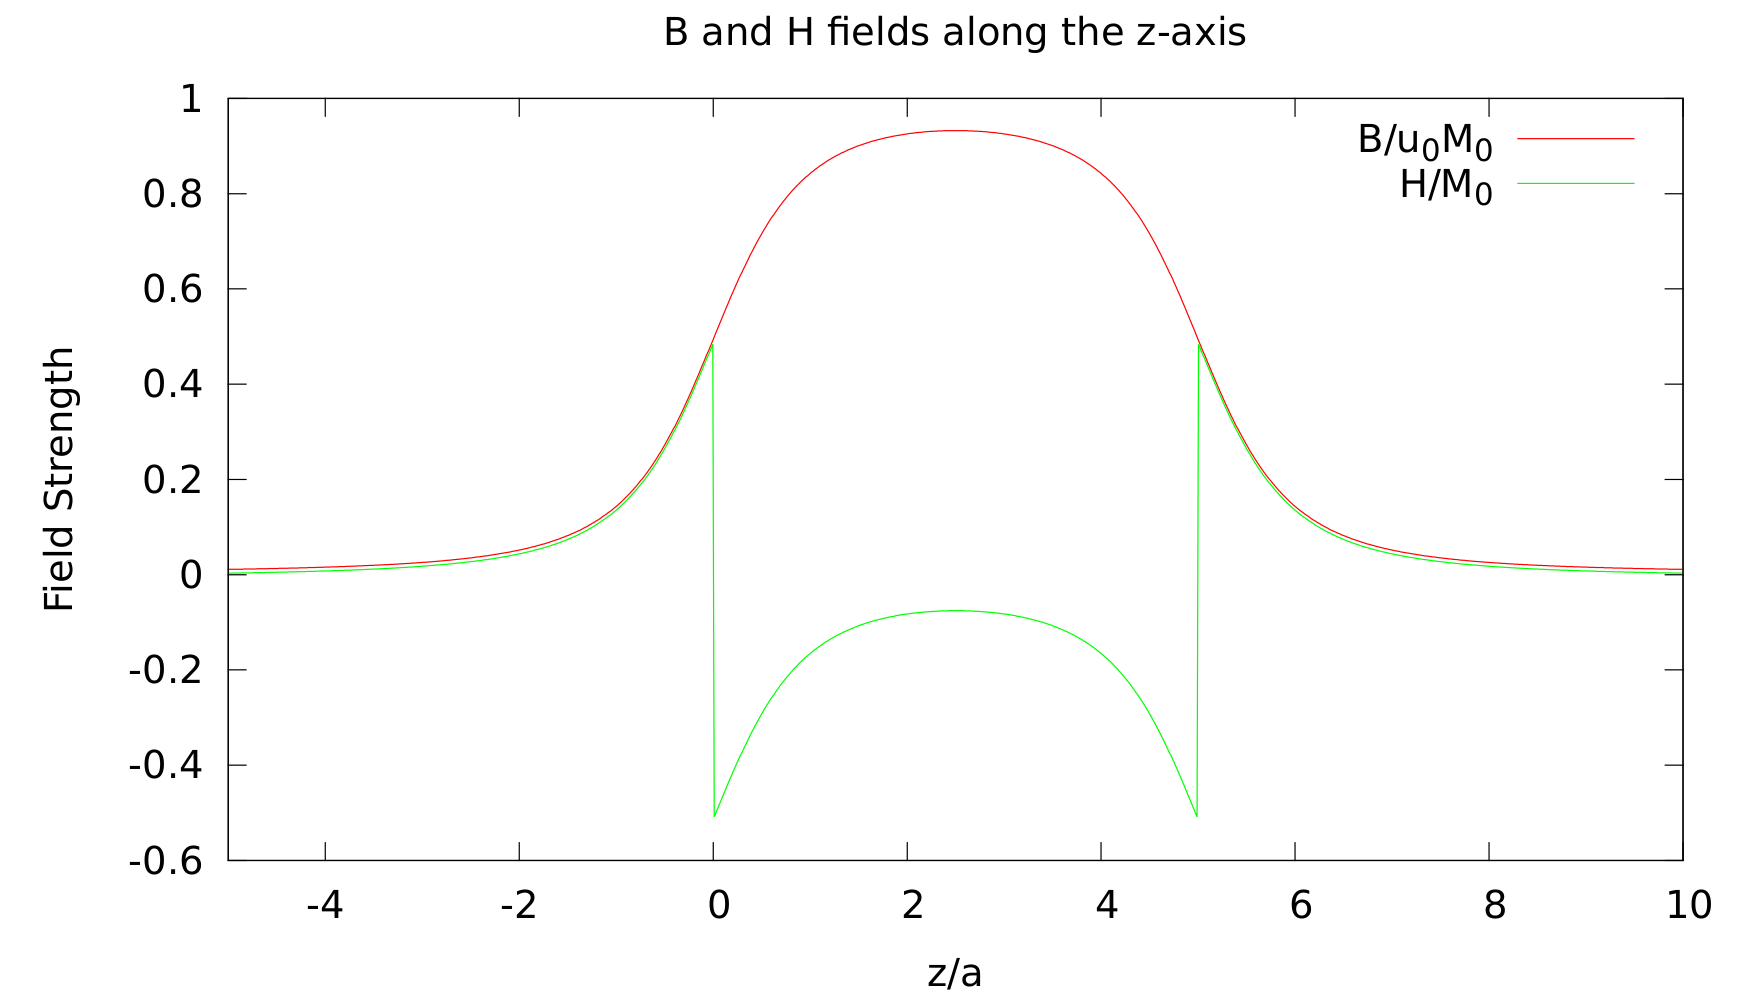
\includegraphics[width=1\textwidth]{5-19-plot.png}
\end{figure}
\end{document}